% Options for packages loaded elsewhere
\PassOptionsToPackage{unicode}{hyperref}
\PassOptionsToPackage{hyphens}{url}
%
\documentclass[
]{book}
\usepackage{amsmath,amssymb}
\usepackage{lmodern}
\usepackage{iftex}
\ifPDFTeX
  \usepackage[T1]{fontenc}
  \usepackage[utf8]{inputenc}
  \usepackage{textcomp} % provide euro and other symbols
\else % if luatex or xetex
  \usepackage{unicode-math}
  \defaultfontfeatures{Scale=MatchLowercase}
  \defaultfontfeatures[\rmfamily]{Ligatures=TeX,Scale=1}
\fi
% Use upquote if available, for straight quotes in verbatim environments
\IfFileExists{upquote.sty}{\usepackage{upquote}}{}
\IfFileExists{microtype.sty}{% use microtype if available
  \usepackage[]{microtype}
  \UseMicrotypeSet[protrusion]{basicmath} % disable protrusion for tt fonts
}{}
\makeatletter
\@ifundefined{KOMAClassName}{% if non-KOMA class
  \IfFileExists{parskip.sty}{%
    \usepackage{parskip}
  }{% else
    \setlength{\parindent}{0pt}
    \setlength{\parskip}{6pt plus 2pt minus 1pt}}
}{% if KOMA class
  \KOMAoptions{parskip=half}}
\makeatother
\usepackage{xcolor}
\IfFileExists{xurl.sty}{\usepackage{xurl}}{} % add URL line breaks if available
\IfFileExists{bookmark.sty}{\usepackage{bookmark}}{\usepackage{hyperref}}
\hypersetup{
  pdftitle={Spatial R Exercise 1},
  pdfauthor={Ben Davies},
  hidelinks,
  pdfcreator={LaTeX via pandoc}}
\urlstyle{same} % disable monospaced font for URLs
\usepackage{color}
\usepackage{fancyvrb}
\newcommand{\VerbBar}{|}
\newcommand{\VERB}{\Verb[commandchars=\\\{\}]}
\DefineVerbatimEnvironment{Highlighting}{Verbatim}{commandchars=\\\{\}}
% Add ',fontsize=\small' for more characters per line
\usepackage{framed}
\definecolor{shadecolor}{RGB}{248,248,248}
\newenvironment{Shaded}{\begin{snugshade}}{\end{snugshade}}
\newcommand{\AlertTok}[1]{\textcolor[rgb]{0.94,0.16,0.16}{#1}}
\newcommand{\AnnotationTok}[1]{\textcolor[rgb]{0.56,0.35,0.01}{\textbf{\textit{#1}}}}
\newcommand{\AttributeTok}[1]{\textcolor[rgb]{0.77,0.63,0.00}{#1}}
\newcommand{\BaseNTok}[1]{\textcolor[rgb]{0.00,0.00,0.81}{#1}}
\newcommand{\BuiltInTok}[1]{#1}
\newcommand{\CharTok}[1]{\textcolor[rgb]{0.31,0.60,0.02}{#1}}
\newcommand{\CommentTok}[1]{\textcolor[rgb]{0.56,0.35,0.01}{\textit{#1}}}
\newcommand{\CommentVarTok}[1]{\textcolor[rgb]{0.56,0.35,0.01}{\textbf{\textit{#1}}}}
\newcommand{\ConstantTok}[1]{\textcolor[rgb]{0.00,0.00,0.00}{#1}}
\newcommand{\ControlFlowTok}[1]{\textcolor[rgb]{0.13,0.29,0.53}{\textbf{#1}}}
\newcommand{\DataTypeTok}[1]{\textcolor[rgb]{0.13,0.29,0.53}{#1}}
\newcommand{\DecValTok}[1]{\textcolor[rgb]{0.00,0.00,0.81}{#1}}
\newcommand{\DocumentationTok}[1]{\textcolor[rgb]{0.56,0.35,0.01}{\textbf{\textit{#1}}}}
\newcommand{\ErrorTok}[1]{\textcolor[rgb]{0.64,0.00,0.00}{\textbf{#1}}}
\newcommand{\ExtensionTok}[1]{#1}
\newcommand{\FloatTok}[1]{\textcolor[rgb]{0.00,0.00,0.81}{#1}}
\newcommand{\FunctionTok}[1]{\textcolor[rgb]{0.00,0.00,0.00}{#1}}
\newcommand{\ImportTok}[1]{#1}
\newcommand{\InformationTok}[1]{\textcolor[rgb]{0.56,0.35,0.01}{\textbf{\textit{#1}}}}
\newcommand{\KeywordTok}[1]{\textcolor[rgb]{0.13,0.29,0.53}{\textbf{#1}}}
\newcommand{\NormalTok}[1]{#1}
\newcommand{\OperatorTok}[1]{\textcolor[rgb]{0.81,0.36,0.00}{\textbf{#1}}}
\newcommand{\OtherTok}[1]{\textcolor[rgb]{0.56,0.35,0.01}{#1}}
\newcommand{\PreprocessorTok}[1]{\textcolor[rgb]{0.56,0.35,0.01}{\textit{#1}}}
\newcommand{\RegionMarkerTok}[1]{#1}
\newcommand{\SpecialCharTok}[1]{\textcolor[rgb]{0.00,0.00,0.00}{#1}}
\newcommand{\SpecialStringTok}[1]{\textcolor[rgb]{0.31,0.60,0.02}{#1}}
\newcommand{\StringTok}[1]{\textcolor[rgb]{0.31,0.60,0.02}{#1}}
\newcommand{\VariableTok}[1]{\textcolor[rgb]{0.00,0.00,0.00}{#1}}
\newcommand{\VerbatimStringTok}[1]{\textcolor[rgb]{0.31,0.60,0.02}{#1}}
\newcommand{\WarningTok}[1]{\textcolor[rgb]{0.56,0.35,0.01}{\textbf{\textit{#1}}}}
\usepackage{longtable,booktabs,array}
\usepackage{calc} % for calculating minipage widths
% Correct order of tables after \paragraph or \subparagraph
\usepackage{etoolbox}
\makeatletter
\patchcmd\longtable{\par}{\if@noskipsec\mbox{}\fi\par}{}{}
\makeatother
% Allow footnotes in longtable head/foot
\IfFileExists{footnotehyper.sty}{\usepackage{footnotehyper}}{\usepackage{footnote}}
\makesavenoteenv{longtable}
\usepackage{graphicx}
\makeatletter
\def\maxwidth{\ifdim\Gin@nat@width>\linewidth\linewidth\else\Gin@nat@width\fi}
\def\maxheight{\ifdim\Gin@nat@height>\textheight\textheight\else\Gin@nat@height\fi}
\makeatother
% Scale images if necessary, so that they will not overflow the page
% margins by default, and it is still possible to overwrite the defaults
% using explicit options in \includegraphics[width, height, ...]{}
\setkeys{Gin}{width=\maxwidth,height=\maxheight,keepaspectratio}
% Set default figure placement to htbp
\makeatletter
\def\fps@figure{htbp}
\makeatother
\setlength{\emergencystretch}{3em} % prevent overfull lines
\providecommand{\tightlist}{%
  \setlength{\itemsep}{0pt}\setlength{\parskip}{0pt}}
\setcounter{secnumdepth}{5}
\usepackage{booktabs}
\ifLuaTeX
  \usepackage{selnolig}  % disable illegal ligatures
\fi
\usepackage[]{natbib}
\bibliographystyle{plainnat}

\title{Spatial R Exercise 1}
\author{Ben Davies}
\date{2022-05-08}

\begin{document}
\maketitle

{
\setcounter{tocdepth}{1}
\tableofcontents
}
\hypertarget{adding-the-sf-package}{%
\chapter{\texorpdfstring{Adding the \texttt{sf} package}{Adding the sf package}}\label{adding-the-sf-package}}

First, we'll include the \texttt{sf} package that we'll use for working with vector data.

\begin{Shaded}
\begin{Highlighting}[]
\FunctionTok{require}\NormalTok{(sf)}
\end{Highlighting}
\end{Shaded}

\begin{verbatim}
## Loading required package: sf
\end{verbatim}

\begin{verbatim}
## Linking to GEOS 3.9.1, GDAL 3.3.2, PROJ 7.2.1; sf_use_s2() is TRUE
\end{verbatim}

Remember that this package is built as an update of the \texttt{sp} package. This uses the \emph{Simple Features} object format, where spatial data are stored as dataframes with a special ``geometry'' column. This makes them more flexible for use by other packages. You can read more about Simple Features \href{http://wiki.gis.com/wiki/index.php/Simple_Features}{here}, and about the history of spatial data handling in R \href{https://link.springer.com/article/10.1007/s10109-020-00336-0}{here}.

\hypertarget{working-with-spatial-data}{%
\chapter{Working with spatial data}\label{working-with-spatial-data}}

\hypertarget{reading-in-a-shapefile}{%
\section{Reading in a shapefile}\label{reading-in-a-shapefile}}

Now that we have access to the \texttt{sf} package, we'll read in a shapefile (south\_africa\_border.shp) with the borders of the countries in southern Africa: South Africa, Lesotho, and Eswatini.

\begin{Shaded}
\begin{Highlighting}[]
\CommentTok{\#Import the south\_africa\_border.shp shapefile. }
\NormalTok{southernAfrica}\OtherTok{\textless{}{-}}\FunctionTok{st\_read}\NormalTok{(}\StringTok{"south\_africa\_border.shp"}\NormalTok{)}
\end{Highlighting}
\end{Shaded}

\begin{verbatim}
## Reading layer `south_africa_border' from data source 
##   `C:\Users\bdav_\Dropbox\Teaching\Spatial R Short Course\Bookdown\Exercise1\south_africa_border.shp' 
##   using driver `ESRI Shapefile'
## Simple feature collection with 3 features and 94 fields
## Geometry type: POLYGON
## Dimension:     XY
## Bounding box:  xmin: 16.46998 ymin: -34.82195 xmax: 32.89308 ymax: -22.12645
## Geodetic CRS:  WGS 84
\end{verbatim}

This dataset comes from \href{www.naturalearthdata.com}{Natural Earth}, and it includes 95 variables about these 3 countries, including population, GDP, country names in other languages, etc. If you wanted to take a look at it in more detail, you could use \texttt{str(southernAfrica)}, but you can also take my word for it.

\hypertarget{plotting-spatial-data}{%
\section{Plotting spatial data}\label{plotting-spatial-data}}

Next we'll use \texttt{plot} and \texttt{st\_geometry} to plot the borders.

\begin{Shaded}
\begin{Highlighting}[]
\CommentTok{\#Plot geometry}
\FunctionTok{plot}\NormalTok{(}\FunctionTok{st\_geometry}\NormalTok{(southernAfrica))}
\end{Highlighting}
\end{Shaded}

\includegraphics{_main_files/figure-latex/unnamed-chunk-3-1.pdf}

While we all probably have a sense of where southern Africa is, it's usually a good idea to include some information about the geography. We'll learn more about making maps later, but for now we can just include the axes to give us latitude and longitude.

\begin{Shaded}
\begin{Highlighting}[]
\CommentTok{\#Plot geometry with axes}
\FunctionTok{plot}\NormalTok{(}\FunctionTok{st\_geometry}\NormalTok{(southernAfrica),}\AttributeTok{axes=}\NormalTok{T)}
\end{Highlighting}
\end{Shaded}

\includegraphics{_main_files/figure-latex/unnamed-chunk-4-1.pdf}

If we want to see the information in the dataset, we could just use the \texttt{plot} function by itself.

\begin{Shaded}
\begin{Highlighting}[]
\FunctionTok{plot}\NormalTok{(southernAfrica)}
\end{Highlighting}
\end{Shaded}

\begin{verbatim}
## Warning: plotting the first 9 out of 94 attributes; use max.plot = 94 to plot
## all
\end{verbatim}

\includegraphics{_main_files/figure-latex/unnamed-chunk-5-1.pdf}

You may notice that this gives us the first nine variables (or columns) in the dataset. Since a vector dataset might contain hundreds of variables, the \texttt{sf} package will stop after 9 plots by default so that R doesn't freak out.
You may also notice that for many of these, there's no differences between these countries. It's probably more useful to target a specific variable of interest. For example, if we want to access the population estimate for each country and plot that, we first need to figure out which variable corresponds to the population. You can get a list of variable names using \texttt{colnames} or just by typing \texttt{southernAfrica\$} into the command line.

\begin{Shaded}
\begin{Highlighting}[]
\FunctionTok{colnames}\NormalTok{(southernAfrica)}
\end{Highlighting}
\end{Shaded}

\begin{verbatim}
##  [1] "featurecla" "scalerank"  "LABELRANK"  "SOVEREIGNT" "SOV_A3"    
##  [6] "ADM0_DIF"   "LEVEL"      "TYPE"       "ADMIN"      "ADM0_A3"   
## [11] "GEOU_DIF"   "GEOUNIT"    "GU_A3"      "SU_DIF"     "SUBUNIT"   
## [16] "SU_A3"      "BRK_DIFF"   "NAME"       "NAME_LONG"  "BRK_A3"    
## [21] "BRK_NAME"   "BRK_GROUP"  "ABBREV"     "POSTAL"     "FORMAL_EN" 
## [26] "FORMAL_FR"  "NAME_CIAWF" "NOTE_ADM0"  "NOTE_BRK"   "NAME_SORT" 
## [31] "NAME_ALT"   "MAPCOLOR7"  "MAPCOLOR8"  "MAPCOLOR9"  "MAPCOLOR13"
## [36] "POP_EST"    "POP_RANK"   "GDP_MD_EST" "POP_YEAR"   "LASTCENSUS"
## [41] "GDP_YEAR"   "ECONOMY"    "INCOME_GRP" "WIKIPEDIA"  "FIPS_10_"  
## [46] "ISO_A2"     "ISO_A3"     "ISO_A3_EH"  "ISO_N3"     "UN_A3"     
## [51] "WB_A2"      "WB_A3"      "WOE_ID"     "WOE_ID_EH"  "WOE_NOTE"  
## [56] "ADM0_A3_IS" "ADM0_A3_US" "ADM0_A3_UN" "ADM0_A3_WB" "CONTINENT" 
## [61] "REGION_UN"  "SUBREGION"  "REGION_WB"  "NAME_LEN"   "LONG_LEN"  
## [66] "ABBREV_LEN" "TINY"       "HOMEPART"   "MIN_ZOOM"   "MIN_LABEL" 
## [71] "MAX_LABEL"  "NE_ID"      "WIKIDATAID" "NAME_AR"    "NAME_BN"   
## [76] "NAME_DE"    "NAME_EN"    "NAME_ES"    "NAME_FR"    "NAME_EL"   
## [81] "NAME_HI"    "NAME_HU"    "NAME_ID"    "NAME_IT"    "NAME_JA"   
## [86] "NAME_KO"    "NAME_NL"    "NAME_PL"    "NAME_PT"    "NAME_RU"   
## [91] "NAME_SV"    "NAME_TR"    "NAME_VI"    "NAME_ZH"    "geometry"
\end{verbatim}

There's a lot of variables here, but once we know the name of the variable we are interested in, we can plot this using brackets to include the variable name:

\begin{Shaded}
\begin{Highlighting}[]
\FunctionTok{plot}\NormalTok{(southernAfrica[}\StringTok{\textquotesingle{}POP\_EST\textquotesingle{}}\NormalTok{])}
\end{Highlighting}
\end{Shaded}

\includegraphics{_main_files/figure-latex/unnamed-chunk-7-1.pdf}

This shows us that, unsurprisingly, there are population differences between South Africa, Lesotho, and Eswatini. But more importantly, it shows that you can import and explore this data using a few lines of code.

\hypertarget{try-it-yourself}{%
\section{Try it yourself!}\label{try-it-yourself}}

Add some code to see if you can do the following with the southern Africa data:

\begin{itemize}
\tightlist
\item
  Figure out which variable/column gives the gross domestic product (GDP) estimate for each country
\item
  Plot the GDP data with latitude/longitude axes
\item
  Can you think of a way to plot the population estimate and GDP side by side (with axes)?
\end{itemize}

\hypertarget{subsetting-data}{%
\chapter{Subsetting data}\label{subsetting-data}}

\hypertarget{adding-more-data}{%
\section{Adding more data}\label{adding-more-data}}

In this step, we'll import some more slightly more interesting data: biomes in southern Africa.

\begin{Shaded}
\begin{Highlighting}[]
\CommentTok{\#Import SABiomes.csv data}
\NormalTok{biomes}\OtherTok{\textless{}{-}}\FunctionTok{st\_read}\NormalTok{(}\StringTok{"SABiomes.shp"}\NormalTok{)}
\end{Highlighting}
\end{Shaded}

\begin{verbatim}
## Reading layer `SABiomes' from data source 
##   `C:\Users\bdav_\Dropbox\Teaching\Spatial R Short Course\Bookdown\Exercise1\SABiomes.shp' 
##   using driver `ESRI Shapefile'
## Simple feature collection with 287 features and 7 fields
## Geometry type: MULTIPOLYGON
## Dimension:     XY
## Bounding box:  xmin: 16.45696 ymin: -34.8334 xmax: 32.89179 ymax: -22.12917
## Geodetic CRS:  WGS 84
\end{verbatim}

This dataset comes from the \href{https://www.sanbi.org/}{South Africa National Biodiversity Institute} and is based on a \href{https://www.cabdirect.org/cabdirect/abstract/20073221934}{2006 classification scheme by Mucina and Rutherford}.

You might notice that when you import this dataset, it reports the following:

\texttt{Geometry\ type:\ MULTIPOLYGON}

The ``multi'' types of geometry isn't something we have seen yet, but you may be familiar with these if you have used other GIS platforms. The main difference between a \texttt{POLYGON} and \texttt{MULTIPOLYGON} geometry is that in a \texttt{POLYGON} geometry, each individual polygon is a distinct feature, while in a \texttt{MULTIPOLYGON} geometry, multiple polygons might be included in a single feature. You could think about it in terms of the main islands of Hawaii:

\includegraphics{hawaii.png}

A\texttt{POLYGON} dataset might have separate features for Oahu, Maui, Kauai, and so on, while a \texttt{MULTIPOLYGON} dataset might have 8 polygons that are all a single feature called ``Hawaii''. For the biomes dataset, some areas may include disconnected components, but are here considered to be a single feature or ``multipolygon''.

Let's use the \texttt{unique} function to take a look at how many different biomes are in this dataset:

\begin{Shaded}
\begin{Highlighting}[]
\CommentTok{\#How many features are in this dataset?}
\FunctionTok{unique}\NormalTok{(biomes}\SpecialCharTok{$}\NormalTok{BIOMENAME)}
\end{Highlighting}
\end{Shaded}

\begin{verbatim}
## [1] "Forests"                   "Grassland"                
## [3] "Savanna"                   "Nama-Karoo"               
## [5] "Desert"                    "Fynbos"                   
## [7] "Indian Ocean Coastal Belt" "Succulent Karoo"          
## [9] "Albany Thicket"
\end{verbatim}

This shows us the names of all 9 of the primary biomes in South Africa. Now we can look at their distribution by plotting them. We probably don't need to plot every variable, so let's just use the \texttt{BIOMECODE} variable to plot by.

\begin{Shaded}
\begin{Highlighting}[]
\CommentTok{\#Plot by biome code}
\FunctionTok{plot}\NormalTok{(biomes[}\StringTok{\textquotesingle{}BIOMECODE\textquotesingle{}}\NormalTok{])}
\end{Highlighting}
\end{Shaded}

\includegraphics{_main_files/figure-latex/unnamed-chunk-10-1.pdf}

Lovely! We should also add axes.

\begin{Shaded}
\begin{Highlighting}[]
\CommentTok{\#Plot by biome code with axes}
\FunctionTok{plot}\NormalTok{(biomes[}\StringTok{\textquotesingle{}BIOMECODE\textquotesingle{}}\NormalTok{],}\AttributeTok{axes=}\NormalTok{T)}
\end{Highlighting}
\end{Shaded}

\includegraphics{_main_files/figure-latex/unnamed-chunk-11-1.pdf}

\hypertarget{subsetting-using-attribute-data}{%
\section{Subsetting using attribute data}\label{subsetting-using-attribute-data}}

Now let's say we're only intrested in the grassland areas. We can use \texttt{subset} to reduce the dataset just to grassland areas.

\begin{Shaded}
\begin{Highlighting}[]
\CommentTok{\#Plot just grasslands}
\NormalTok{grassland}\OtherTok{\textless{}{-}}\FunctionTok{subset}\NormalTok{(biomes,BIOMENAME}\SpecialCharTok{==}\StringTok{"Grassland"}\NormalTok{)}
\FunctionTok{plot}\NormalTok{(}\FunctionTok{st\_geometry}\NormalTok{(grassland))}
\end{Highlighting}
\end{Shaded}

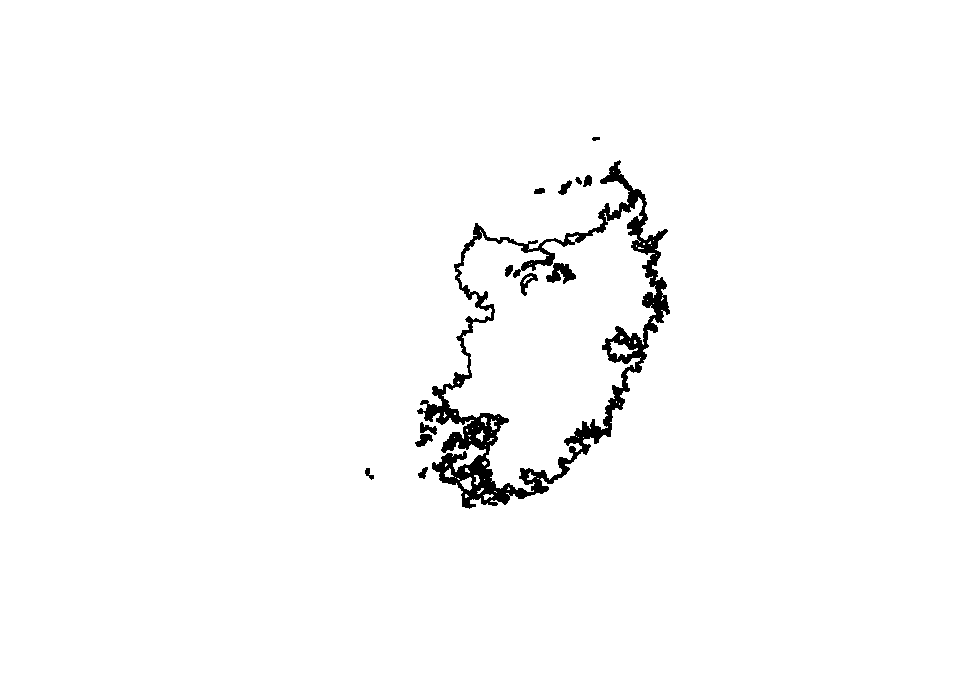
\includegraphics{_main_files/figure-latex/unnamed-chunk-12-1.pdf}

Again, let's include the axes, and let's also make the color light green.

\begin{Shaded}
\begin{Highlighting}[]
\CommentTok{\#Print the grasslands green with axes}
\FunctionTok{plot}\NormalTok{(}\FunctionTok{st\_geometry}\NormalTok{(grassland),}\AttributeTok{axes=}\NormalTok{T,}\AttributeTok{col=}\StringTok{"light green"}\NormalTok{)}
\end{Highlighting}
\end{Shaded}

\includegraphics{_main_files/figure-latex/unnamed-chunk-13-1.pdf}

Looking good so far!

\hypertarget{try-it-yourself-1}{%
\section{Try it yourself!}\label{try-it-yourself-1}}

Modify the blank code chunk below to see if you can do the following with the biomes data:

\begin{itemize}
\tightlist
\item
  Subset the data so that it is just the savanna biome
\item
  Plot this and choose a complementary color. If you're not sure what the options are for colors, \href{http://www.stat.columbia.edu/~tzheng/files/Rcolor.pdf}{try this document}.
\item
  Change the type and thickness of the lines used to draw the features with the \texttt{lty} and \texttt{lwd} arguments. These take numeric values and default to 1. See what happens when you change these.
\item
  See if you can plot the geometry of the southern Africa, and then add the savanna.
\end{itemize}

\hypertarget{creating-sf-objects-from-table-data}{%
\chapter{\texorpdfstring{Creating \texttt{sf} objects from table data}{Creating sf objects from table data}}\label{creating-sf-objects-from-table-data}}

\hypertarget{adding-csv-data}{%
\section{Adding CSV data}\label{adding-csv-data}}

Now let's say we have some point data and we want to add it to the map. However, in this case we've got it stored as a comma-separated values (CSV) file. Let's use \texttt{read.csv} to read the data in, and \texttt{class} to look at the object class.

\begin{Shaded}
\begin{Highlighting}[]
\CommentTok{\#Import the SARadiocarbon.csv data}
\NormalTok{c14table}\OtherTok{\textless{}{-}}\FunctionTok{read.csv}\NormalTok{(}\StringTok{"SARadiocarbon.csv"}\NormalTok{)}
\FunctionTok{class}\NormalTok{(c14table)}
\end{Highlighting}
\end{Shaded}

\begin{verbatim}
## [1] "data.frame"
\end{verbatim}

These data are radiocarbon dates from the \href{https://www.cambridge.org/core/journals/antiquity/article/abs/an-archaeological-radiocarbon-database-for-southern-africa/26FE99E995C4507015704D552CB0C196}{South African Radiocarbon Database}. The \texttt{read.csv} function reads this in as a dataframe only, so it isn't being treated as an sf object just yet. Let's take a look at the dataframe using the \texttt{head} function, which gives a preview of the first 6 rows:

\begin{Shaded}
\begin{Highlighting}[]
\CommentTok{\#Take a look at the first 6 rows}
\FunctionTok{head}\NormalTok{(c14table)}
\end{Highlighting}
\end{Shaded}

\begin{verbatim}
##         SITE SITE_CODE LATITUDE LONGITUDE      COUNTRY PROVINCE_DISTRICT RFZ
## 1 Thula Mela       TUM  -22.431    31.194 South Africa           Limpopo   S
## 2 Thula Mela       TUM  -22.431    31.194 South Africa           Limpopo   S
## 3 Thula Mela       TUM  -22.431    31.194 South Africa           Limpopo   S
## 4 Thula Mela       TUM  -22.431    31.194 South Africa           Limpopo   S
## 5 Thula Mela       TUM  -22.431    31.194 South Africa           Limpopo   S
## 6 Thula Mela       TUM  -22.431    31.194 South Africa           Limpopo   S
##           BIOME CONTEXT        TECHNIQUE MATERIAL      SPECIES   LAB_ID DATE
## 1 Savanna Biome         conventional 14C charcoal              Pta-6079  480
## 2 Savanna Biome         conventional 14C charcoal              Pta-7107  530
## 3 Savanna Biome         conventional 14C charcoal              Pta-7103  390
## 4 Savanna Biome         conventional 14C charcoal              Pta-7105  560
## 5 Savanna Biome         conventional 14C     bone Homo sapiens Pta-7276  370
## 6 Savanna Biome         conventional 14C     bone Homo sapiens Pta-7243  520
##   UNCERTAINTY ARCH_PERIOD ARCH_SUBPERIOD SAMPLE_CONTEXT  SITE_TYPE DELTA_13
## 1          30    Iron Age                               settlement       NA
## 2          30    Iron Age                               settlement       NA
## 3          35    Iron Age                               settlement       NA
## 4          35    Iron Age                               settlement       NA
## 5          40    Iron Age                               settlement       NA
## 6          40    Iron Age                               settlement       NA
##        REFCODE   NOTES
## 1 vogel2000rds   Khami
## 2 vogel2000rds Mutamba
## 3 vogel2000rds   Khami
## 4 vogel2000rds Mutamba
## 5 vogel2000rds   Khami
## 6 vogel2000rds   Khami
\end{verbatim}

Among the columns in this dataset is one called \texttt{BIOME}, which tells us from which biome the date was recovered. There are more than 2000 dates in the set, but there probably aren't that many biomes in the dataset. Again, we can use \texttt{unique} to get a list of the ones included here.

\begin{Shaded}
\begin{Highlighting}[]
\CommentTok{\#Get unique biome names}
\FunctionTok{unique}\NormalTok{(c14table}\SpecialCharTok{$}\NormalTok{BIOME)}
\end{Highlighting}
\end{Shaded}

\begin{verbatim}
##  [1] "Savanna Biome"             "Grassland Biome"          
##  [3] "Succulent Karoo Biome"     "Azonal Vegetation"        
##  [5] "Desert Biome"              "Nama-Karoo Biome"         
##  [7] "Fynbos Biome"              "Thicket Biome"            
##  [9] "Forests"                   "Indian Ocean Coastal Belt"
## [11] ""
\end{verbatim}

While there are some minor differences, these match up pretty well with the names from our biomes shapefile. If we wanted just the dates from the grasslands, we could subset the data using this column.

\begin{Shaded}
\begin{Highlighting}[]
\CommentTok{\#Get the grassland dates}
\NormalTok{c14grass}\OtherTok{\textless{}{-}}\FunctionTok{subset}\NormalTok{(c14table,BIOME}\SpecialCharTok{==}\StringTok{"Grassland Biome"}\NormalTok{)}
\FunctionTok{unique}\NormalTok{(c14grass}\SpecialCharTok{$}\NormalTok{BIOME)}
\end{Highlighting}
\end{Shaded}

\begin{verbatim}
## [1] "Grassland Biome"
\end{verbatim}

Terrific. Now we want to make this usable with \texttt{sf}. Lucky for us this is already spatial data: coordinates are stored in the columns \texttt{LONGITUDE} and \texttt{LATITUDE}. We can use these columns as arguments with the \texttt{st\_as\_sf} to coerce the dataframe to a point dataset.

\begin{Shaded}
\begin{Highlighting}[]
\CommentTok{\#Convert to point object}
\NormalTok{c14points}\OtherTok{\textless{}{-}}\FunctionTok{st\_as\_sf}\NormalTok{(c14grass,}\AttributeTok{coords=}\FunctionTok{c}\NormalTok{(}\StringTok{"LONGITUDE"}\NormalTok{,}\StringTok{"LATITUDE"}\NormalTok{),}\AttributeTok{remove=}\ConstantTok{FALSE}\NormalTok{)}
\end{Highlighting}
\end{Shaded}

Notice that we added an argument to the \texttt{st\_as\_sf} function that says \texttt{remove=FALSE}. This means that when we use \texttt{LONGITUDE} and \texttt{LATITUDE} to generate our geometry, we don't remove these columns. These will come in handy later on. For now, let's check on the class of this new object.

\begin{Shaded}
\begin{Highlighting}[]
\FunctionTok{class}\NormalTok{(c14points)}
\end{Highlighting}
\end{Shaded}

\begin{verbatim}
## [1] "sf"         "data.frame"
\end{verbatim}

OK, now it's in the sf class, so we can add it to our map.

\begin{Shaded}
\begin{Highlighting}[]
\CommentTok{\#Add to plot}
\FunctionTok{plot}\NormalTok{(}\FunctionTok{st\_geometry}\NormalTok{(grassland),}\AttributeTok{axes=}\NormalTok{T,}\AttributeTok{col=}\StringTok{"light green"}\NormalTok{)}
\FunctionTok{plot}\NormalTok{(}\FunctionTok{st\_geometry}\NormalTok{(c14points),}\AttributeTok{add=}\NormalTok{T)}
\end{Highlighting}
\end{Shaded}

\includegraphics{_main_files/figure-latex/unnamed-chunk-20-1.pdf}

\hypertarget{subsetting-using-location-data}{%
\section{Subsetting using location data}\label{subsetting-using-location-data}}

Not bad! Notice that one point just east of the edge of the grassland boundary? It's not clear what's happened there: it could be from a site that is in a transition zone, or maybe was mislabeled by the data authors. Whatever it is, let's say we don't want to include that point. We can use subset again, but this time we only want to include points that are inside our grassland object. We'll use \texttt{st\_bbox} to get the extent of the grassland object:

\begin{Shaded}
\begin{Highlighting}[]
\FunctionTok{st\_bbox}\NormalTok{(grassland)}
\end{Highlighting}
\end{Shaded}

\begin{verbatim}
##      xmin      ymin      xmax      ymax 
##  22.33500 -33.06480  31.66951 -22.99997
\end{verbatim}

These values are the maximum and minimum x and y coordinates for the grassland object. We can see that the \texttt{xmax}, or the longitude that is the furthest to the east, is 31.66951. We can use \texttt{subset} and the \texttt{LONGITUDE} column we kept to pare it down.

\begin{Shaded}
\begin{Highlighting}[]
\NormalTok{c14points2}\OtherTok{\textless{}{-}}\FunctionTok{subset}\NormalTok{(c14points, LONGITUDE }\SpecialCharTok{\textless{}} \FloatTok{31.66951}\NormalTok{)}
\end{Highlighting}
\end{Shaded}

And then we plot again..

\begin{Shaded}
\begin{Highlighting}[]
\CommentTok{\#Add to plot}
\FunctionTok{plot}\NormalTok{(}\FunctionTok{st\_geometry}\NormalTok{(grassland),}\AttributeTok{axes=}\NormalTok{T,}\AttributeTok{col=}\StringTok{"light green"}\NormalTok{)}
\FunctionTok{plot}\NormalTok{(}\FunctionTok{st\_geometry}\NormalTok{(c14points2),}\AttributeTok{add=}\NormalTok{T)}
\end{Highlighting}
\end{Shaded}

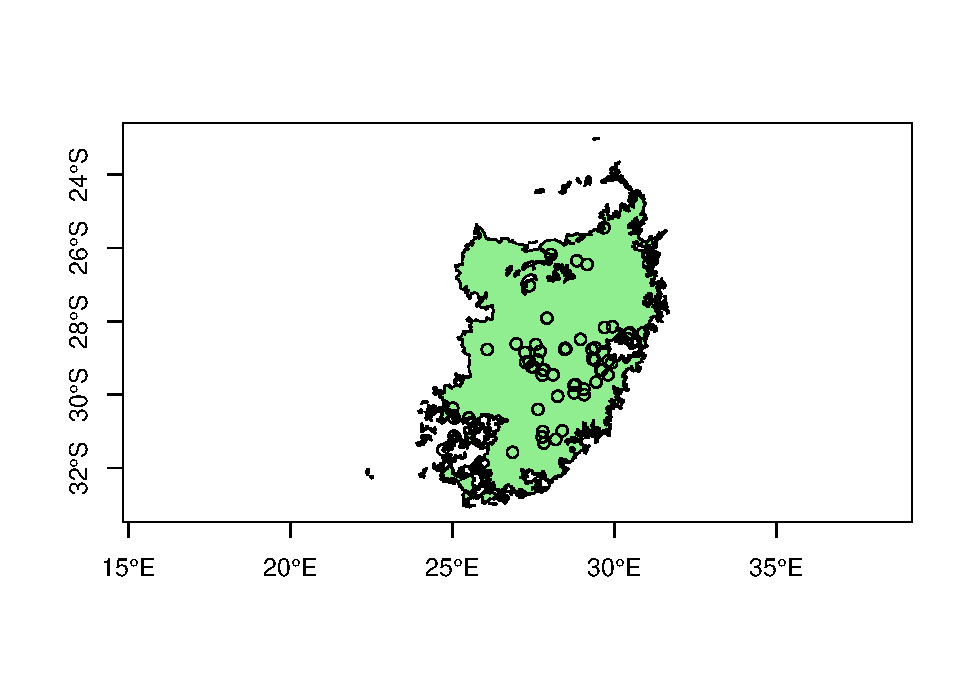
\includegraphics{_main_files/figure-latex/unnamed-chunk-23-1.pdf}

Fixed! This is an example of \emph{spatial subsetting}. In this case, since there was only one point we wanted to prune and we had the \texttt{LONGITUDE} data handy, it was pretty easy to do it this way. But if the , we'd probably want to find a way to crop the points using the biome shape itself. This is something we'll cover in more detail in another session.

\hypertarget{creating-sf-objects-from-scratch}{%
\chapter{\texorpdfstring{Creating \texttt{sf} objects from scratch}{Creating sf objects from scratch}}\label{creating-sf-objects-from-scratch}}

\hypertarget{making-spatial-data}{%
\section{Making spatial data}\label{making-spatial-data}}

Lastly, let's add some data we make ourselves. Let's say we have a section of grassland we want to use as a study area. To do this, we're going to make a square polygon using longitude/latitude coordinates. First, we use \texttt{list} and \texttt{rbind} to create a list object with a matrix of coordinate pairs:

\begin{Shaded}
\begin{Highlighting}[]
\CommentTok{\#Make polygon list}
\NormalTok{polygonList }\OtherTok{=} \FunctionTok{list}\NormalTok{(}\FunctionTok{rbind}\NormalTok{(}\FunctionTok{c}\NormalTok{(}\FloatTok{26.5}\NormalTok{, }\SpecialCharTok{{-}}\DecValTok{28}\NormalTok{), }\FunctionTok{c}\NormalTok{(}\FloatTok{29.5}\NormalTok{, }\SpecialCharTok{{-}}\DecValTok{28}\NormalTok{), }\FunctionTok{c}\NormalTok{(}\FloatTok{29.5}\NormalTok{, }\SpecialCharTok{{-}}\DecValTok{30}\NormalTok{), }\FunctionTok{c}\NormalTok{(}\FloatTok{26.5}\NormalTok{, }\SpecialCharTok{{-}}\DecValTok{30}\NormalTok{), }\FunctionTok{c}\NormalTok{(}\FloatTok{26.5}\NormalTok{, }\SpecialCharTok{{-}}\DecValTok{28}\NormalTok{)))}
\end{Highlighting}
\end{Shaded}

Next, we trainslate this list into a polygon object with \texttt{st\_polygon}, and then a feature collection with \texttt{st\_sfc}:

\begin{Shaded}
\begin{Highlighting}[]
\NormalTok{polygonObject}\OtherTok{\textless{}{-}}\FunctionTok{st\_polygon}\NormalTok{(polygonList)}
\NormalTok{polygonCollection}\OtherTok{\textless{}{-}}\FunctionTok{st\_sfc}\NormalTok{(polygonObject)}
\end{Highlighting}
\end{Shaded}

Now we generate some ``data'' to include. Since it's only one feature we're making, we can just give it a feature number of 1. We turn this into a dataframe, and then combine them with the feature collection to make a new simple features dataset with \texttt{st\_sf}:

\begin{Shaded}
\begin{Highlighting}[]
\NormalTok{featureNum}\OtherTok{\textless{}{-}}\FunctionTok{c}\NormalTok{(}\DecValTok{1}\NormalTok{)}
\NormalTok{data}\OtherTok{\textless{}{-}}\FunctionTok{data.frame}\NormalTok{(featureNum)}
\NormalTok{polygonData}\OtherTok{\textless{}{-}}\FunctionTok{st\_sf}\NormalTok{(data,polygonCollection)}
\end{Highlighting}
\end{Shaded}

Finally, we need to tell it what coordinate system we are using. The EPSG coordinate system code for the WGS84 Geographic Coordinate System (the standard used in GPS) is 4326. We can assign this easily using \texttt{st\_crs}, and use the same function to check it:

\begin{Shaded}
\begin{Highlighting}[]
\FunctionTok{st\_crs}\NormalTok{(polygonData) }\OtherTok{\textless{}{-}} \DecValTok{4326}
\FunctionTok{st\_crs}\NormalTok{(polygonData)}
\end{Highlighting}
\end{Shaded}

\begin{verbatim}
## Coordinate Reference System:
##   User input: EPSG:4326 
##   wkt:
## GEOGCRS["WGS 84",
##     DATUM["World Geodetic System 1984",
##         ELLIPSOID["WGS 84",6378137,298.257223563,
##             LENGTHUNIT["metre",1]]],
##     PRIMEM["Greenwich",0,
##         ANGLEUNIT["degree",0.0174532925199433]],
##     CS[ellipsoidal,2],
##         AXIS["geodetic latitude (Lat)",north,
##             ORDER[1],
##             ANGLEUNIT["degree",0.0174532925199433]],
##         AXIS["geodetic longitude (Lon)",east,
##             ORDER[2],
##             ANGLEUNIT["degree",0.0174532925199433]],
##     USAGE[
##         SCOPE["Horizontal component of 3D system."],
##         AREA["World."],
##         BBOX[-90,-180,90,180]],
##     ID["EPSG",4326]]
\end{verbatim}

Lastly, we want to plot our newly created study area polygon with our other data:

\begin{Shaded}
\begin{Highlighting}[]
\CommentTok{\#Add to plot}
\FunctionTok{plot}\NormalTok{(}\FunctionTok{st\_geometry}\NormalTok{(grassland),}\AttributeTok{axes=}\NormalTok{T,}\AttributeTok{col=}\StringTok{"light green"}\NormalTok{)}
\FunctionTok{plot}\NormalTok{(}\FunctionTok{st\_geometry}\NormalTok{(c14points2),}\AttributeTok{add=}\NormalTok{T)}
\FunctionTok{plot}\NormalTok{(}\FunctionTok{st\_geometry}\NormalTok{(polygonData),}\AttributeTok{add=}\NormalTok{T)}
\end{Highlighting}
\end{Shaded}

\includegraphics{_main_files/figure-latex/unnamed-chunk-28-1.pdf}

\hypertarget{writing-to-file}{%
\section{Writing to file}\label{writing-to-file}}

And if we want to export our new data as a shapefile, we can use \texttt{st\_write}:

\begin{Shaded}
\begin{Highlighting}[]
\CommentTok{\#Export it to shapefile (remove the \# to run this code)}
\CommentTok{\#st\_write(polygonData,"sampleArea.shp",driver="ESRI shapefile")}
\end{Highlighting}
\end{Shaded}

\hypertarget{bring-it-all-together}{%
\chapter{Bring it all together!}\label{bring-it-all-together}}

Try to write code to do the following on your own:

\begin{itemize}
\tightlist
\item
  Load the biomes shapefile and radiocarbon data
\item
  Subset both of these to the Fynbos Biome
\item
  Make a histogram using the dates in the fynbos subset of the radiocarbon data using the \texttt{hist} function
\item
  Create another subset of the fynbos radiocarbon data that includes Pleistocene dates only (dates older than 11700 BP)
\item
  Plot the following:

  \begin{itemize}
  \tightlist
  \item
    The fynbos biome in the color of your choosing (not red or black) with axes
  \item
    The fynbos radiocarbon dates as small, black circles (you can change the size of the points using the \texttt{cex} argument)
  \item
    Pleistocene fynbos radiocarbon dates as larger, red filled circles (you can change the symbols using the \texttt{pch} argument)
  \end{itemize}
\end{itemize}

  \bibliography{book.bib,packages.bib}

\end{document}
